\documentclass[a4paper,11pt]{article}
\input{/home/tof/Documents/Cozy/latex-include/preambule_lua.tex}
\newcommand{\showprof}{show them}  % comment this line if you don't want to see todo environment
\fancyhead[L]{DNS}
\newdate{madate}{10}{09}{2020}
%\fancyhead[R]{\displaydate{madate}} %\today
\fancyhead[R]{Seconde - SNT}
%\fancyhead[R]{Première - NSI}
%\fancyhead[R]{Terminale - NSI}
\fancyfoot[L]{~\\Christophe Viroulaud}
\AtEndDocument{\label{lastpage}}
\fancyfoot[C]{\textbf{Page \thepage/\pageref{lastpage}}}
\fancyfoot[R]{\includegraphics[width=2cm,align=t]{/home/tof/Documents/Cozy/latex-include/cc.png}}

\begin{document}
\begin{Form}
\section{Problématique}
Sur internet chaque machine est repérée par son adresse IP. Par exemple, le moteur de recherche de Google est hébergé sur un ordinateur (\emph{serveur}) qui a pour adresse 172.217.19.227.
\begin{activite}
Dans la barre d'adresse du navigateur (Firefox, Chrome...) entrer l'adresse IP 172.217.19.227 puis valider.
\end{activite}
Cependant il est plus simple de demander aux utilisateurs de retenir \emph{www.google.com} qu'une suite de nombres.
\begin{center}
\shadowbox{\parbox{14cm}{\centering Comment retrouver l'adresse IP d'un ordinateur à partir de l'adresse du site?}}
\end{center}
\section{Contexte historique}
Au début des années 1980 un fichier \emph{(hosts.txt)} contenait les correspondances entre les noms et les adresses IP. Ce fichier était copié intégralement sur chaque ordinateur du réseau.
\begin{activite}
Pour quelles raisons ce système ne pourrait pas être mise en place aujourd'hui?
\end{activite}
Un autre système a rapidement été mis en place: le \emph{Domain Name System (DNS)}. Paul Mockapetris publie la conception du système en 1983. Il fut rapidement adopté pour internet.
\section{Fonctionnement du DNS}
\subsection{Serveurs dédiés}
Plutôt que de stocker les adresses sur chaque ordinateur personnel, des machines spécialisées \emph{(serveurs DNS)} sont répartis sur le réseau mondial. Elles recensent toutes les correspondances \emph{IP}\leftrightarrow\emph{adresse web}.\\
Que se passe-t-il alors quand l'utilisateur entre l'adresse web dans le navigateur (figure \ref{barre})?
\begin{figure}[!h]
\centering

\includegraphics[width=15cm]{ressources/barre.png}
\captionof{figure}{Barre d'adresse du navigateur}
\label{barre}
\end{figure}

La \emph{résolution d'une adresse web} se déroule en plusieurs étapes:
\begin{enumerate}
\item L'ordinateur personnel envoie une requête au serveur DNS:\\ \guill{Quelle est l'adresse IP de \emph{www.google.com}?}
\item Le serveur répond: \guill{Il s'agit de 172.217.19.227}
\item L'ordinateur personnel demande alors à la machine 172.217.19.227: \guill{Envoie moi la page web correspondante.}
\item La machine 172.217.19.227 renvoie le contenu de la page.
\end{enumerate}
\begin{activite}
\begin{enumerate}
\item À l'aide du site \url{http://www.mon-ip.com/adresse-ip-site-internet.php}, retrouver l'IP du site \url{https://lyceejaydebeaufort.fr/}.
\item Sur la figure \ref{requete}, placer des flèches numérotées qui correspondent à la résolution d'une adresse web décrite précédemment.
\end{enumerate}

\end{activite}
\begin{figure}[!h]
\centering

\includegraphics[width=10cm]{ressources/serveur-dns.png}
\captionof{figure}{Requête DNS}
\label{requete}
\end{figure}

\subsection{Construction d'une adresse}
Le serveur DNS est en réalité composé de plusieurs machines qui ont chacune leur rôle. Le système des noms de domaine consiste en une hiérarchie dont le sommet est appelé la racine. On représente cette dernière par un point (figure \ref{hierarchie}). L'adresse est lue de droite à gauche. 
\begin{figure}[!h]
\centering
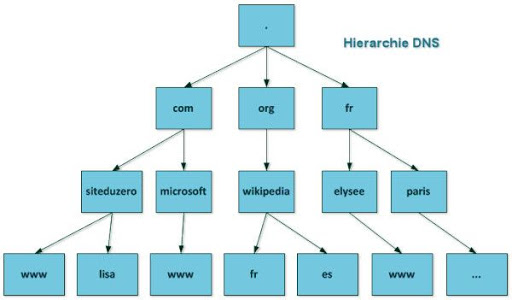
\includegraphics[width=10cm]{ressources/hierarchie.jpg}
\captionof{figure}{Hierarchie DNS}
\label{hierarchie}
\end{figure}

Pour \emph{résoudre} l'adresse
\begin{center}
\url{https://fr.wikipedia.org}
\end{center}
la première machine délègue au serveur qui gère le domaine \emph{org}. Celui-ci délègue au serveur qui s'occupe du domaine \emph{wikipedia.org}. Enfin une dernière délégation est accomplie vers le serveur qui gère l'adresse IP du sous-domaine \emph{fr.wikipedia.org}.
\begin{activite}
Sur la figure \ref{hierarchie} tracer les délégations accomplies pour résoudre l'adresse \url{https://www.elysee.fr}.
\end{activite}
\end{Form}
\end{document}